
\documentclass[12pt,a4paper]{article}
\usepackage{geometry}
 \geometry{
 a4paper,
 total={170mm,257mm},
 left=20mm,
 top=20mm,
 }
\usepackage[utf8]{inputenc}
\usepackage[T1]{fontenc}
%\geometry{verbose,tmargin=3cm,bmargin=2cm,lmargin=2cm,rmargin=2cm,headheight=2cm,headsep=2cm,footskip=2cm}
\usepackage{array}
\usepackage{float}
\usepackage{textcomp}
\usepackage{slashed}
\usepackage{amsmath}
\usepackage{graphicx}
\usepackage{tikz}

\makeatletter

%%%%%%%%%%%%%%%%%%%%%%%%%%%%%% LyX specific LaTeX commands.
%% Because html converters don't know tabularnewline
\providecommand{\tabularnewline}{\\}

\makeatother

\usepackage{babel}
\begin{document}
\section{Oppgaver}
\subsection{fysikk}
\begin{enumerate}
\item Fyll ut manglende felter\\
	\huge
\begin{tabular}{|c|c|c|}
\hline 
$10^{n}$ & Prefiks  & Symbol\tabularnewline
\hline 
\hline 
$10^{12}$ & tera & \tabularnewline
\hline 
$10^{9}$ &  & G\tabularnewline
\hline 
$10^{6}$ & mega & \tabularnewline
\hline 
 & kilo  & k\tabularnewline
\hline 
 & milli  & \tabularnewline
\hline 
$10^{-6}$ & mikro  & \textmu{}\tabularnewline
\hline 
$10^{-9}$ &  & n\tabularnewline
\hline 
 & pico  & p\tabularnewline
\hline 
\end{tabular}
\normalsize
\item Hvor mange elektroner kan det være i valensskallet?
\vskip 5pt 

\begin{tikzpicture}
	\draw[step=0.5cm,gray!20,very thin]  grid (17,1) ;
\end{tikzpicture}
\vskip 2.5pt 
\item Hvor mange elektroner kan det være i valensskallet til:

\begin{enumerate}
\item Ledere
\vskip 5pt 

\begin{tikzpicture}
	\draw[step=0.5cm,gray!20,very thin]  grid (16,1) ;
\end{tikzpicture}
\vskip 2.5pt 
\item Halvledere 
\vskip 5pt 

\begin{tikzpicture}
	\draw[step=0.5cm,gray!20,very thin]  grid (16,1) ;
\end{tikzpicture}
\vskip 2.5pt 
\item Isolaorer 
\vskip 5pt 

\begin{tikzpicture}
	\draw[step=0.5cm,gray!20,very thin]  grid (16,1) ;
\end{tikzpicture}
\vskip 2.5pt 
\end{enumerate}
\item Hva vil det si at et stoff har elektrisk ladning?
\vskip 5pt 

\begin{tikzpicture}
	\draw[step=0.5cm,gray!20,very thin]  grid (17,1) ;
\end{tikzpicture}
\vskip 2.5pt 
\item Hva er benevnelsen og enheten til spenning?
\vskip 5pt 

\begin{tikzpicture}
	\draw[step=0.5cm,gray!20,very thin]  grid (17,1) ;
\end{tikzpicture}
\vskip 2.5pt 
\item Hva er benevnelsen og enheten til strøm?
\vskip 5pt 

\begin{tikzpicture}
	\draw[step=0.5cm,gray!20,very thin]  grid (17,1) ;
\end{tikzpicture}
\vskip 2.5pt 
\item Hva er benevnelsen og enheten til resistans?
\vskip 5pt 

\begin{tikzpicture}
	\draw[step=0.5cm,gray!20,very thin]  grid (17,1) ;
\end{tikzpicture}
\vskip 2.5pt 
\item Tegn symbolet for en resistor (motstand).
\vskip 5pt 

\begin{tikzpicture}
	\draw[step=0.5cm,gray!20,very thin]  grid (17,1) ;
\end{tikzpicture}
\vskip 2.5pt 
\item Nevn tre måter å produsere elektrisk spenning på. 
\vskip 5pt 

\begin{tikzpicture}
	\draw[step=0.5cm,gray!20,very thin]  grid (17,1) ;
\end{tikzpicture}
\vskip 2.5pt 
\item Hva oppnår vi ved å parallellkoble to batterier?
\vskip 5pt 

\begin{tikzpicture}
	\draw[step=0.5cm,gray!20,very thin]  grid (17,1) ;
\end{tikzpicture}
\vskip 2.5pt 
\item Hva oppnår vi ved å seriekoble to batterier?
\vskip 5pt 

\begin{tikzpicture}
	\draw[step=0.5cm,gray!20,very thin]  grid (17,1) ;
\end{tikzpicture}
\vskip 2.5pt 
\end{enumerate}

\subsubsection{Ohms lov}

I oppgave 3-13 må du tegne kretsen. 
\begin{enumerate}
\item Ohms lov skrives på følgende tre måter:
\vskip 5pt 

\begin{tikzpicture}
	\draw[step=0.5cm,gray!20,very thin]  grid (17,1) ;
\end{tikzpicture}
\vskip 2.5pt 
\item Hvor stor spenning ligger det over en resistans på $22\Omega$ når det går 10A gjennom den?
\vskip 5pt 

\begin{tikzpicture}
	\draw[step=0.5cm,gray!20,very thin]  grid (17,1) ;
\end{tikzpicture}
\vskip 2.5pt 
\item Hvor stor strøm går det gjennom en resistans på $44\Omega$ når det ligger en spenning på 220V over den?
\vskip 5pt 
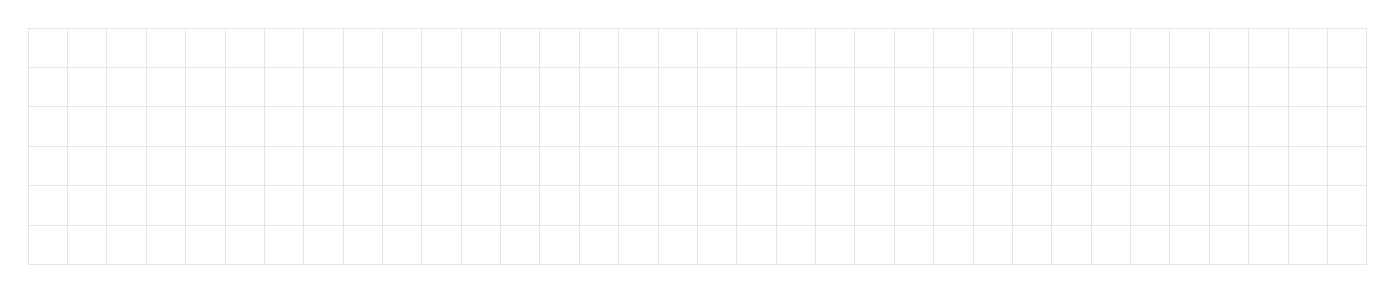
\begin{tikzpicture}
	\draw[step=0.5cm,gray!20,very thin]  grid (17,3) ;
\end{tikzpicture}
\vskip 2.5pt 
\item Hvor stor resistansverdi har en motstand når det går en strøm på 2.0A gjennom den og spenningen over den er 220V?
\vskip 5pt 
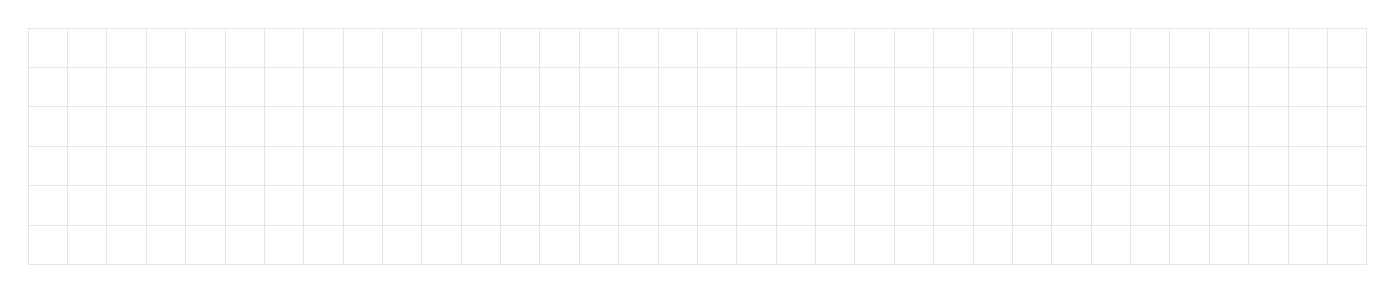
\begin{tikzpicture}
	\draw[step=0.5cm,gray!20,very thin]  grid (17,3) ;
\end{tikzpicture}
\vskip 2.5pt 
\item Det ligger 1.5V over en motstand på $4.5\Omega$, hvor stor strøm går det i den?
\vskip 5pt 
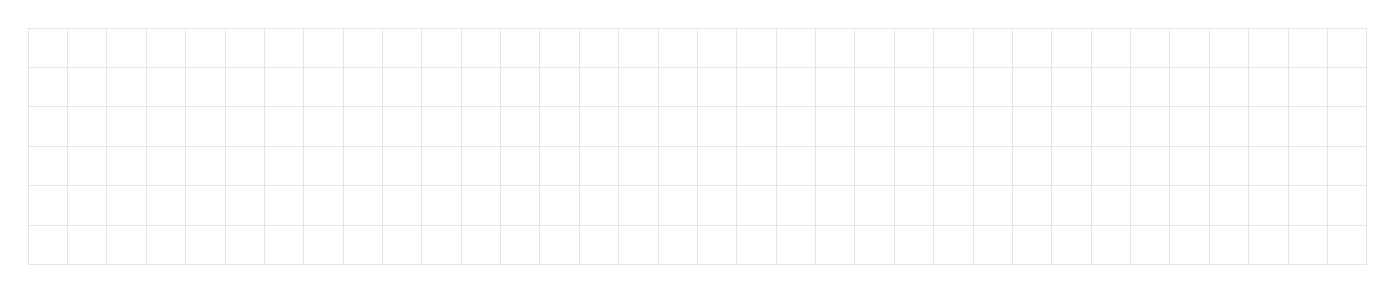
\begin{tikzpicture}
	\draw[step=0.5cm,gray!20,very thin]  grid (17,3) ;
\end{tikzpicture}
\vskip 2.5pt 
\item En elektrisk ovn bruker 8.0A ved spenningen 220V. Hvor stor resistans har den?
\vskip 5pt 
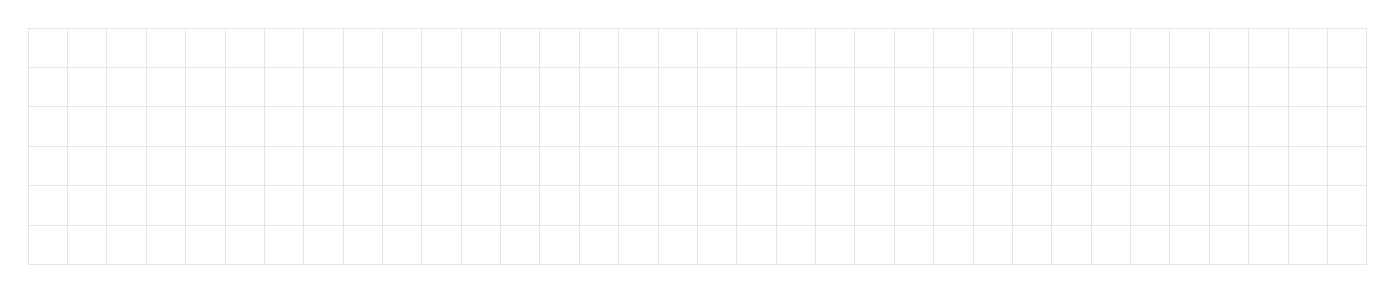
\begin{tikzpicture}
	\draw[step=0.5cm,gray!20,very thin]  grid (17,3) ;
\end{tikzpicture}
\vskip 2.5pt 
\item Hvor stor spenning kreves for å drive 5A gjennom en resistans på $20\Omega$? 
\vskip 5pt 
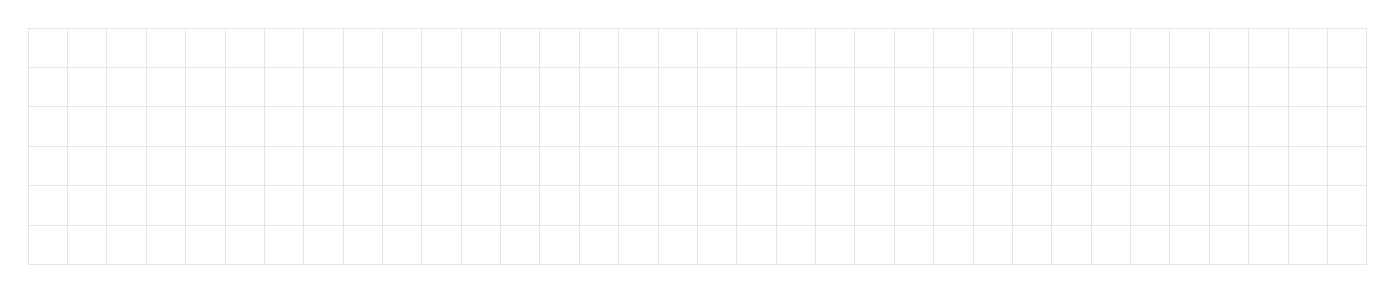
\begin{tikzpicture}
	\draw[step=0.5cm,gray!20,very thin]  grid (17,3) ;
\end{tikzpicture}
\vskip 2.5pt 
\item Hvor stor er spenningen over en resistans på $300\Omega$ når det går en strøm på 8.0A gjennom den?
\vskip 5pt 
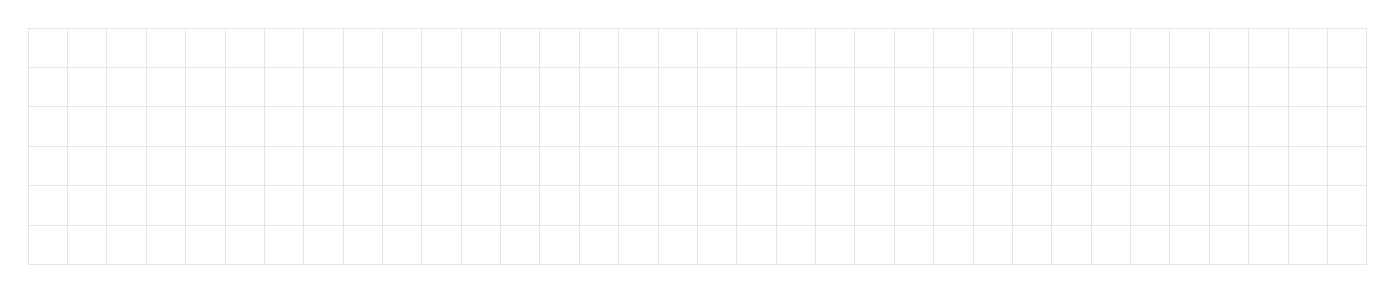
\begin{tikzpicture}
	\draw[step=0.5cm,gray!20,very thin]  grid (17,3) ;
\end{tikzpicture}
\vskip 2.5pt 
\item Det flyter en strøm på 3 A gjennom en resistans på 150$\Omega$ beregn spenningen over resistansen. 
\vskip 5pt 
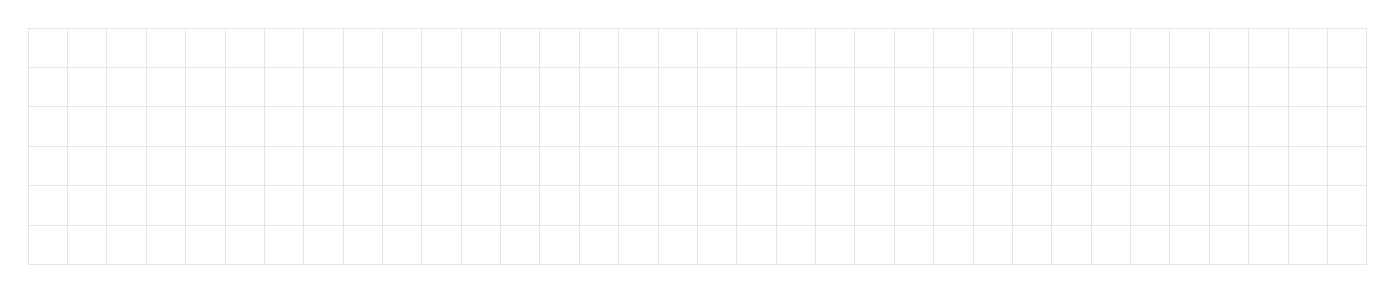
\begin{tikzpicture}
	\draw[step=0.5cm,gray!20,very thin]  grid (17,3) ;
\end{tikzpicture}
\vskip 2.5pt 
\item En resistans på $75\Omega$ blir påtrykt en spenning på 230v. Hva blir strømmen gjennom resistansen? 
\vskip 5pt 
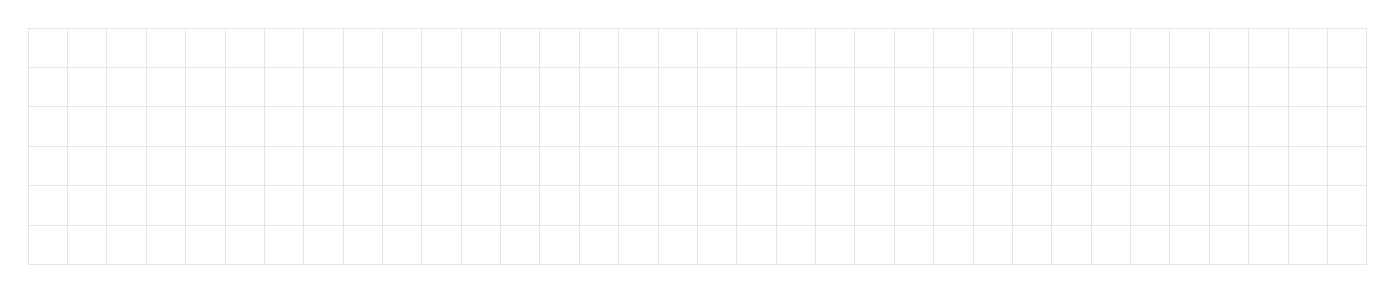
\begin{tikzpicture}
	\draw[step=0.5cm,gray!20,very thin]  grid (17,3) ;
\end{tikzpicture}
\vskip 2.5pt 
\item Hvor stor verdi har en motstand når det går en strøm på 2A gjennom den og spenningen over den er 220v? 
\vskip 5pt 
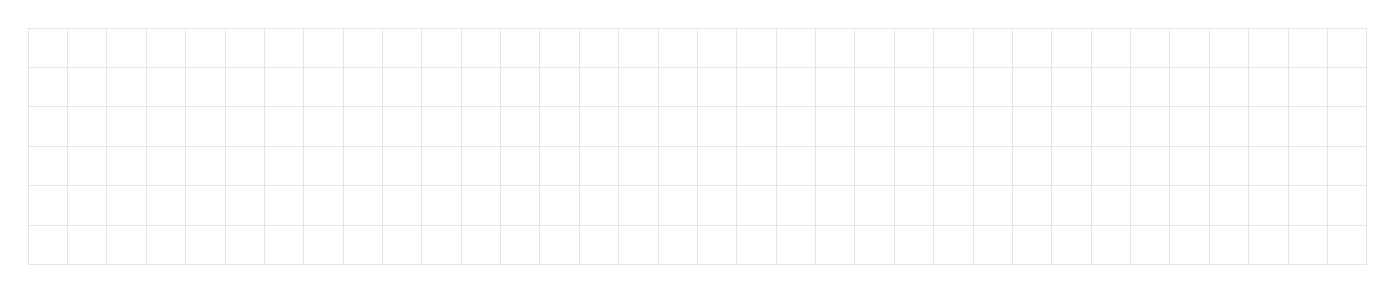
\begin{tikzpicture}
	\draw[step=0.5cm,gray!20,very thin]  grid (17,3) ;
\end{tikzpicture}
\vskip 2.5pt 
\item Hvor stor strøm går det gjennom en resistans på $22\Omega$ når det ligger en spenning på 220v over den? 
\vskip 5pt 
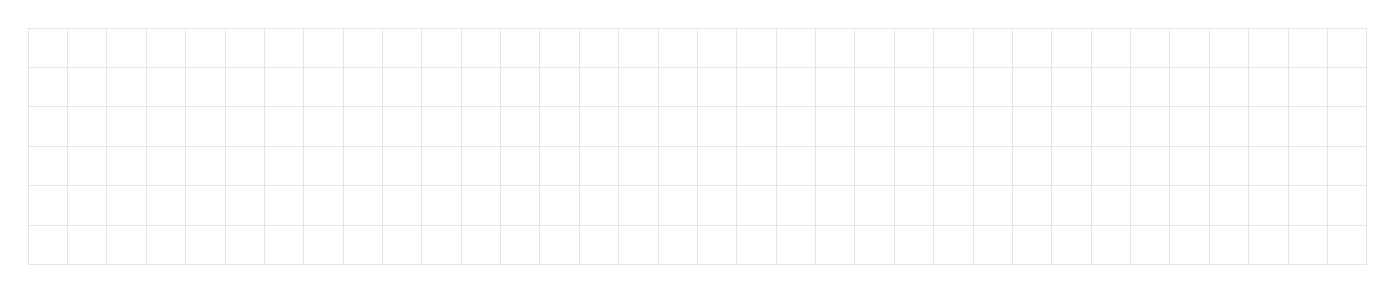
\begin{tikzpicture}
	\draw[step=0.5cm,gray!20,very thin]  grid (17,3) ;
\end{tikzpicture}
\vskip 2.5pt 
\item Hva skjer i en krets bestående av en spenningskilde og en resistans når:

\begin{enumerate}
\item Spenningen tredobles
\vskip 5pt 

\begin{tikzpicture}
	\draw[step=0.5cm,gray!20,very thin]  grid (16,1) ;
\end{tikzpicture}
\vskip 2.5pt 
\item Spenningen reduseres med 75\%
\vskip 5pt 

\begin{tikzpicture}
	\draw[step=0.5cm,gray!20,very thin]  grid (16,1) ;
\end{tikzpicture}
\vskip 2.5pt 
\item Resistansen dobbles
\vskip 5pt 

\begin{tikzpicture}
	\draw[step=0.5cm,gray!20,very thin]  grid (16,1) ;
\end{tikzpicture}
\vskip 2.5pt 
\item Resistansen reduseres med 35\%
\vskip 5pt 

\begin{tikzpicture}
	\draw[step=0.5cm,gray!20,very thin]  grid (16,1) ;
\end{tikzpicture}
\vskip 2.5pt 
\item Spenningen dobbles og resistansen dobbles
\vskip 5pt 

\begin{tikzpicture}
	\draw[step=0.5cm,gray!20,very thin]  grid (16,1) ;
\end{tikzpicture}
\vskip 2.5pt 
\end{enumerate}
\end{enumerate}

\newpage
\subsubsection{Seriekretser}
\begin{enumerate}
\item Seriekobling av resistanser

\begin{enumerate}
\item Skriv formelen for erstatningsresistanden (totalresistansen) i en seriekobling av resistanser.
\\
\begin{tikzpicture}
	\draw[step=0.5cm,gray!20,very thin]  grid (15,1) ;
\end{tikzpicture}
\item Du skal seriekoble $R_{1}=5\Omega$, $R_{2}=15\Omega$ og $R_{3}=20\Omega$. Hvor stor er totalresistansen?
\\
\begin{tikzpicture}
	\draw[step=0.5cm,gray!20,very thin]  grid (15,1) ;
\end{tikzpicture}
\item Totalresistansen i en seriekobling er $5000\Omega$. Seriekoblingen består av tre resistanser på $1000\Omega$ og en ukjent resistans.Hvor stor er en ukjente resistansen?
\\
\begin{tikzpicture}
	\draw[step=0.5cm,gray!20,very thin]  grid (15,2) ;
\end{tikzpicture}
\item Du skal seriekoble $R_{1}=5k\Omega,\,R_{2}=100\Omega,\,R_{3}=0.4k\Omega\,og\,R_{4}=500\Omega$. Hvor stor er totalresistansen?
\\
\begin{tikzpicture}
	\draw[step=0.5cm,gray!20,very thin]  grid (15,2) ;
\end{tikzpicture}
\end{enumerate}
\item Kirchhoffs spennings lov omhandler delspenninger og spenningskilder.
(i seriekobling) den sier at $U=U_{R1}+U_{R2}+U_{Rn}$....... 

\begin{enumerate}
\item Tre motstander er seriekoblet. Med et voltmeter måles spenningene over motstandene til $U_{R1}=15V,\,U_{R2}=5V,\,og\,U_{R3}=30V$ Hvor stor er den tilførte spenningen?
\\
\begin{tikzpicture}
	\draw[step=0.5cm,gray!20,very thin]  grid (15,2) ;
\end{tikzpicture}
\item Strømmen gjennom motstandern $R_{1}$ i oppgave a) er 10mA. Hvor stor strøm går det gjennom de andre motstandene?
\\
\begin{tikzpicture}
	\draw[step=0.5cm,gray!20,very thin]  grid (15,2) ;
\end{tikzpicture}
\item Hvor store er resistansverdiene i de tre motstandene?
\\
\begin{tikzpicture}
	\draw[step=0.5cm,gray!20,very thin]  grid (15,2) ;
\end{tikzpicture}
\end{enumerate}
\item Vi seriekobler $R_{1}=200\Omega,\,R_{2}=100\Omega,\,R_{3}=50\Omega$
og $R_{4}$. Når vi kobler 200 til seriekoblingens ytterpunkter, går
det 0.5A i kretsen. 

\begin{enumerate}
\item Hvor stor strøm går det gjennom $R_{1},\,R_{2},\,R_{4},$ og $R_{4}$ 
\\
\begin{tikzpicture}
	\draw[step=0.5cm,gray!20,very thin]  grid (15,2) ;
\end{tikzpicture}
\item Hvor stor er kretsens totalresistans?
\\
\begin{tikzpicture}
	\draw[step=0.5cm,gray!20,very thin]  grid (15,2) ;
\end{tikzpicture}
\item Hvor stor er $R_{4}$?
\\
\begin{tikzpicture}
	\draw[step=0.5cm,gray!20,very thin]  grid (15,2) ;
\end{tikzpicture}
\item Hvor stor spenning ligger det over hver av motstandene?
\\
\begin{tikzpicture}
	\draw[step=0.5cm,gray!20,very thin]  grid (15,2) ;
\end{tikzpicture}
\end{enumerate}
%\item To resistanser på 100$\Omega$ og 120$\Omega$ er seriekoplet til
%en spenning på 110 V. Hva blir total resistans, strømmen og spenningsfallene
%over hver resistans? 
%\item Tre resistanser er seriekoplet den minste er på $4\Omega$ og neste
%er dobbelt så stor og den tredje er dobbelt så stor som den andre.
%Hva blir total resistans, strømmen og spenningsfallene over hver resistans
%når påtrykt spenning er 100 V?
%\item Fire resistanser er seriekoplet. Verdiene som er i kretsen er: $R_{t}=200\Omega\,R_{1}=50\Omega\,R_{2}=20\Omega\,R_{3}=10\Omega$
%og $U_{R4}=240V$
%
%\begin{enumerate}
%\item Beregn resistansen $R_{4}$.
%\item Hvilken strøm går det i kretsen?
%\item Finn total- og delspenningene.
%\end{enumerate}
%\item Tre resistanser blir seriekoplet for å gi forskjellige spenninger.
%Resistansene er på 150\foreignlanguage{english}{$\Omega$} , 300$\Omega$
%og 450$\Omega$ . Hovedspenning er 230 V, finn spenningene som kretsen
%kan gi utenom hovedspenningen
%\item Gjennom en seriekrets går det en strøm på 4 A. Det er to resistanser
%i kretsen den ene er tre ganger større enn den andre. 
%
%\begin{enumerate}
%\item Hvor store er resistansene når spenningen er 200 V
%\item Spenningen blir forandret til 150 V. Hva blir strømmen og delspenningene
%med den nye hovedspenningen.
%\end{enumerate}
\end{enumerate}

\newpage
\subsubsection{Parallellkobling}
\begin{enumerate}
\item ~

\begin{enumerate}
\item Skriv den generelle formelen for erstatningsresistansen (totalresistansen) for en parallellkobing av resistanser.
\\
\begin{tikzpicture}
	\draw[step=0.5cm,gray!20,very thin]  grid (15,2) ;
\end{tikzpicture}
\item Hvor stor blir totalresistansen i forhold til resistansene i parallellkoblingen?
\\
\begin{tikzpicture}
	\draw[step=0.5cm,gray!20,very thin]  grid (15,2) ;
\end{tikzpicture}
\item Dersom to motstandere er parallellkoblet, hvordan er forholdet mellom spenningen over dem?
\\
\begin{tikzpicture}
	\draw[step=0.5cm,gray!20,very thin]  grid (15,2) ;
\end{tikzpicture}
\item Du parallellkobler like store resistanser. Hvor stor blir totalresistansen. 
\\
\begin{tikzpicture}
	\draw[step=0.5cm,gray!20,very thin]  grid (15,2) ;
\end{tikzpicture}
\end{enumerate}
\item Kirchhoffs strøm lov omhandler greinstrømmer. 

\begin{enumerate}
\item Skriv den som formel.
\\
\begin{tikzpicture}
	\draw[step=0.5cm,gray!20,very thin]  grid (15,2) ;
\end{tikzpicture}
\item Du parallellkobler to resistander med verdiene $4\Omega\,og\,6\Omega$. Hvor stor blir totalresistansen til koblingen?
\\
\begin{tikzpicture}
	\draw[step=0.5cm,gray!20,very thin]  grid (15,2) ;
\end{tikzpicture}
\item Spenningen over kretsen er 24V. Hvor stor strøm trekker koblingen fra spenningskilden?
\\
\begin{tikzpicture}
	\draw[step=0.5cm,gray!20,very thin]  grid (15,2) ;
\end{tikzpicture}
\item Hvor stor strøm går det igjennom hver av resistansene?
\\
\begin{tikzpicture}
	\draw[step=0.5cm,gray!20,very thin]  grid (15,2) ;
\end{tikzpicture}
\end{enumerate}
\item Øker eller minker resistansen i en parallellkobling ettervert som en kobler til fler og fler resistanser?
\\
\begin{tikzpicture}
	\draw[step=0.5cm,gray!20,very thin]  grid (15,2) ;
\end{tikzpicture}
\item Den totale resistansen i en parallellkobling er alltid mindre en?
\\
\begin{tikzpicture}
	\draw[step=0.5cm,gray!20,very thin]  grid (15,2) ;
\end{tikzpicture}
\item To resistanser er parallellkoplet $25\Omega$ og $50\Omega$. Resistansene er tilkoplet en spenning på 110 V. Hva blir total resistans, hovedstrøm og grenstrømmene?
\\\begin{tikzpicture}
	\draw[step=0.5cm,gray!20,very thin]  grid (15,2) ;
\end{tikzpicture}
\item Vi skal lage en strømdeler som deler den innkomne strømmen i tre like store deler.
\\\begin{tikzpicture}
	\draw[step=0.5cm,gray!20,very thin]  grid (15,2) ;
\end{tikzpicture}

\begin{enumerate}
\item Tegn skjema for denne koblingen
\\\begin{tikzpicture}
	\draw[step=0.5cm,gray!20,very thin]  grid (15,2) ;
\end{tikzpicture}
\item Dersom strømdeleren kobles til 240V. Er den innkomne strømmen 12A. Hvor stor er strømdelerens totale resistans. 
\\\begin{tikzpicture}
	\draw[step=0.5cm,gray!20,very thin]  grid (15,2) ;
\end{tikzpicture}
\item Hvor stor er resistansen i de tre strømgreinene?
\\\begin{tikzpicture}
	\draw[step=0.5cm,gray!20,very thin]  grid (15,2) ;
\end{tikzpicture}
\item Om vi kobler tli enda en resistans i parallell med de tre vi har, hvordan går det da med strømmen fra spenningskilden? Øker den, avtar den eller blir den uforandret?
\\\begin{tikzpicture}
	\draw[step=0.5cm,gray!20,very thin]  grid (15,2) ;
\end{tikzpicture}
\end{enumerate}
\item Tre resistanser er parallellkoplet til en spenning på 300 V. $R_{1}=12\Omega,\,R_{2}=18\Omega,\,R_{3}=22\Omega$. Finn total resistans, grenstrømmer og hovedstrøm.
\\\begin{tikzpicture}
	\draw[step=0.5cm,gray!20,very thin]  grid (15,2) ;
\end{tikzpicture}
%\item Tre resistanser er parallellkoplet og har lik ohmverdi. Resistansene er tilkoplet en spenning på 240 V og de utvikler en total effekt på 5,0 kW.
%\\\begin{tikzpicture}
%	\draw[step=0.5cm,gray!20,very thin]  grid (15,2) ;
%\end{tikzpicture}
%
%\begin{enumerate}
%\item Hvor stor blir hver enkelt resistans?
%\\\begin{tikzpicture}
%	\draw[step=0.5cm,gray!20,very thin]  grid (15,2) ;
%\end{tikzpicture}
%\item Beregn alle grenstrømmer.
%\\\begin{tikzpicture}
%	\draw[step=0.5cm,gray!20,very thin]  grid (15,2) ;
%\end{tikzpicture}
%\end{enumerate}
%\item Vi har en krets som vist
%
%\begin{enumerate}
%\item Hvor stor er den totale resistansen i kretsen?
%\\\begin{tikzpicture}
%	\draw[step=0.5cm,gray!20,very thin]  grid (15,2) ;
%\end{tikzpicture}
%\item Hvor stor er kretsens hovedstrøm?
%\\\begin{tikzpicture}
%	\draw[step=0.5cm,gray!20,very thin]  grid (15,2) ;
%\end{tikzpicture}
%\item Hvor stor er greinstrømmen gjennom $R_{1}$?
%\\\begin{tikzpicture}
%	\draw[step=0.5cm,gray!20,very thin]  grid (15,2) ;
%\end{tikzpicture}
%\item Hvor stor er greinstrømmen gjennom $R_{2}$?\\
%\\\begin{tikzpicture}
%	\draw[step=0.5cm,gray!20,very thin]  grid (15,2) ;
%\end{tikzpicture}
%\includegraphics[width=9cm]{./parallell1.pdf}
%\end{enumerate}
%\item Tre resistanser er parallellkoplet. Følgende verdier er oppgitt i
%kretsen: $R_{1}=50\Omega,\,R_{2}=70\Omega,\,I_{R3}=4.25A\,og\,U=170V$
%
%\begin{enumerate}
%\item Beregn $R_{3}$.
%\item Finn grenstrømmene og hovedstrøm.
%\item Hvilken effekt utvikler kretsen og hver resistans?
%\end{enumerate}
%\item Ti resistanser som er koplet i parallell er på $50\Omega$ hver og
%blir tilkoplet en spenning på 110 V.
%
%\begin{enumerate}
%\item Hvor stor blir total resistans?
%\item Hva blir hovedstrømmen og grenstrømmene?
%\item Hovedstrømmen skal reduseres til det halve, hvor mange resistanser
%à $50\Omega$ må parallellkoples. Vis ved regning.
%\end{enumerate}
\end{enumerate}
\newpage
\subsubsection{Kombinerte kretser}
\begin{enumerate}
\item Vi har en krets som vist i figur \ref{fig:-22}. Regn ut:\\

\begin{enumerate}
\item Koblingens totale resistans
\\\begin{tikzpicture}
	\draw[step=0.5cm,gray!20,very thin]  grid (15,2) ;
\end{tikzpicture}
\item Spenningen over $R_{4}$
\\\begin{tikzpicture}
	\draw[step=0.5cm,gray!20,very thin]  grid (15,2) ;
\end{tikzpicture}
\item Spenningen over parallellkoblingen
\\\begin{tikzpicture}
	\draw[step=0.5cm,gray!20,very thin]  grid (15,2) ;
\end{tikzpicture}
\item Greinstrømmene i kretsen\\
\\\begin{tikzpicture}
	\draw[step=0.5cm,gray!20,very thin]  grid (15,2) ;
\end{tikzpicture}
\begin{figure}[H]
\noindent \begin{centering}
\includegraphics[scale=0.75]{./kombinert1.pdf}
\par\end{centering}
\caption{\label{fig:-22}}
\end{figure}
\end{enumerate}
\item Vi har en krets som vist i figur \ref{fig:-2}. Regn ut:

\begin{enumerate}
\item Kretsens totale resistans
\\\begin{tikzpicture}
	\draw[step=0.5cm,gray!20,very thin]  grid (15,2) ;
\end{tikzpicture}
\item Kretsens hovedstrøm
\\\begin{tikzpicture}
	\draw[step=0.5cm,gray!20,very thin]  grid (15,2) ;
\end{tikzpicture}
\item Spenningen over hver av motstanderene
\\\begin{tikzpicture}
	\draw[step=0.5cm,gray!20,very thin]  grid (15,2) ;
\end{tikzpicture}
\item Kretsens greinstrømmer\\
\\\begin{tikzpicture}
	\draw[step=0.5cm,gray!20,very thin]  grid (15,2) ;
\end{tikzpicture}
\begin{figure}[H]
\noindent \begin{centering}
\includegraphics[scale=0.75]{./kombinert2.pdf}
\par\end{centering}
\caption{\label{fig:-2}}
\end{figure}
\end{enumerate}
%\item To paralellkoblede resistanser på 50$\Omega$ og 70$\Omega$ blir
%koblet i serie med tre parallell koblede resistanser på 60$\Omega$,
%70$\Omega$ og 80$\Omega$. Kretsen blir koblet til en spenning på
%230V. 
%
%\begin{enumerate}
%\item Regn ut total resistans.
%\\\begin{tikzpicture}
%	\draw[step=0.5cm,gray!20,very thin]  grid (15,2) ;
%\end{tikzpicture}
%\item Beregn alle spenningsfallene (delspenningene). 
%\\\begin{tikzpicture}
%	\draw[step=0.5cm,gray!20,very thin]  grid (15,2) ;
%\end{tikzpicture}
%\item Finn greinstrømmene i kretsen. 
%\\\begin{tikzpicture}
%	\draw[step=0.5cm,gray!20,very thin]  grid (15,2) ;
%\end{tikzpicture}
%\end{enumerate}
%\item Vi har en krets som vist
%
%\begin{enumerate}
%\item Finn total resistans.
%\\\begin{tikzpicture}
%	\draw[step=0.5cm,gray!20,very thin]  grid (15,2) ;
%\end{tikzpicture}
%\item Beregn alle del spenningene. 
%\\\begin{tikzpicture}
%	\draw[step=0.5cm,gray!20,very thin]  grid (15,2) ;
%\end{tikzpicture}
%\item Hva blir hovedstrøm og greinstrømene i parallellkoblingen?\\
%\\\begin{tikzpicture}
%	\draw[step=0.5cm,gray!20,very thin]  grid (15,2) ;
%\end{tikzpicture}
%\\
%\includegraphics[scale=0.6]{./kombinert3.pdf}
%\end{enumerate}
\end{enumerate}

\newpage
\subsubsection{Energi og Effekt}
\begin{enumerate}
\item Symboler og enheter

\begin{enumerate}
\item Hvilken enhet og hvilken størrelsesbokstav brukes for elektrisk energi?
\\\begin{tikzpicture}
	\draw[step=0.5cm,gray!20,very thin]  grid (15,2) ;
\end{tikzpicture}
\item Hvordan uttrykkes energi ved hjelp av spenning, strøm og tid?
\\\begin{tikzpicture}
	\draw[step=0.5cm,gray!20,very thin]  grid (15,2) ;
\end{tikzpicture}
\item Hvilken enhet og hvilken størrelsesbokstav brukes for elektrisk effekt?
\\\begin{tikzpicture}
	\draw[step=0.5cm,gray!20,very thin]  grid (15,2) ;
\end{tikzpicture}
\item Skriv sammenhengen mellom effekt og energi
\\\begin{tikzpicture}
	\draw[step=0.5cm,gray!20,very thin]  grid (15,2) ;
\end{tikzpicture}
\end{enumerate}
\item Varianter av effektformelen

\begin{enumerate}
\item Skriv effektformelen ved hjelp av spenning og strøm
\\\begin{tikzpicture}
	\draw[step=0.5cm,gray!20,very thin]  grid (15,2) ;
\end{tikzpicture}
\item Skriv effektformelen ved hjelp av spenning og resistans
\\\begin{tikzpicture}
	\draw[step=0.5cm,gray!20,very thin]  grid (15,2) ;
\end{tikzpicture}
\item Skriv effektformelen ved hjelp av strøm og resistans
\\\begin{tikzpicture}
	\draw[step=0.5cm,gray!20,very thin]  grid (15,2) ;
\end{tikzpicture}
\item En motstand er merket 1k$\Omega$/1/4W. Hvor stor strøm kan det maksimalt
\\\begin{tikzpicture}
	\draw[step=0.5cm,gray!20,very thin]  grid (15,2) ;
\end{tikzpicture}
gå i denne motstanden uten at den blir ødelagt?
\end{enumerate}
\item Fyll ut de strørrelsene som mangler i tabellen\\
	\LARGE
\begin{tabular}{|>{\centering}p{2.5cm}|>{\centering}p{2.5cm}|>{\centering}p{2.5cm}|>{\centering}p{2.5cm}|>{\centering}p{2.5cm}|}
\hline 
nr.  & U & R & I & P\tabularnewline
\hline 
\hline 
1 & 1.5V & 100$\Omega$ &  & \tabularnewline
\hline 
2 & 4.5V &  & 0.3A & \tabularnewline
\hline 
3 &  & 200$\Omega$ & 1.1A & \tabularnewline
\hline 
4 & 220V &  & 10A & \tabularnewline
\hline 
5 & 12V &  &  & 45W\tabularnewline
\hline 
6 &  &  & 9.5A & 2 000W\tabularnewline
\hline 
7 & 220V &  &  & 40W\tabularnewline
\hline 
8 & 12V & 120k$\Omega$ &  & \tabularnewline
\hline 
9 & 9V &  &  & 3W\tabularnewline
\hline 
10 &  &  & 1mA & 1W\tabularnewline
\hline 
\end{tabular}
\normalsize
\item Vi har en krets som vist.

\begin{enumerate}
\item Hvor stor er kretsens totale resistans?
\\\begin{tikzpicture}
	\draw[step=0.5cm,gray!20,very thin]  grid (15,2) ;
\end{tikzpicture}
\item Hvor stor strøm går det ut fra spenningskilden og hver stor er greinstrømmene
\\\begin{tikzpicture}
	\draw[step=0.5cm,gray!20,very thin]  grid (15,2) ;
\end{tikzpicture}
\item Hvor stor spenning ligger det over hver av resistansene?
\\\begin{tikzpicture}
	\draw[step=0.5cm,gray!20,very thin]  grid (15,2) ;
\end{tikzpicture}
\item Hvor stor er kretsens totale effektomsetning?
\\\begin{tikzpicture}
	\draw[step=0.5cm,gray!20,very thin]  grid (15,2) ;
\end{tikzpicture}
\item Alle motstandene kan tåle 0.25W. En av motstandene blir ødelagt. Hvilken
motstand er det?
\\\begin{tikzpicture}
	\draw[step=0.5cm,gray!20,very thin]  grid (15,2) ;
\end{tikzpicture}
\end{enumerate}
%\includegraphics[scale=0.5]{./kombinert4.pdf}
%\item Studer teiningen. $U=4.5v\,;\,R_{1}=47\Omega\,;\,R_{2}=56\Omega\,;\,R_{3}=120\Omega$
%
%\begin{enumerate}
%\item Hvor stor er kretsens totale resistans?
%\item Hvor stor strøm går det gjennom hver av motstandene?
%\item Hvor stor effekt omsettes det i hver motstand?
%\item Vi kobler en ny motstand $R_{4}=39\Omega$ i parallell med $R_{1}$.
%Hvor stor spenning vil det nå ligge over hver av motstandene?\\
%\includegraphics[scale=0.5]{./kombinert5.pdf}
%\end{enumerate}
%\item Vi har tre motstandere med følgende resistansverdier: \foreignlanguage{english}{$R_{1}=100\Omega\,;\,R_{2}=220\Omega\,;\,R_{3}=560\Omega$}.
%Alle motstandene tåler en effekt på maks. $\frac{1}{4}W$. Motstandene
%parallellkobles og kobles til en spenning på 6v. 
%
%\begin{enumerate}
%\item Beregn kretsens totale resistans.
%\item Beregn den strømmen som går gjennom hver av motstandene. 
%\item Det viser seg at en av motstandene blir varm og begynner å ryke. Hvilken
%motstander er det, og hva er årsaken?
%\item For å bedre på det forholdet som er nevnt i c, kobles det en motstand
%i serie med kretsen. Hvor stor resistansverdi må $R_{4}$ minst ha
%for at ingen av motstandene skal bli for varme?
%\end{enumerate}
%\item Den totale resistansen i kretsen er $1316\Omega.$
%
%\begin{enumerate}
%\item Hvor stor er $R_{3}$?
%\item Hvor stor strøm går det igjennom hver av motstandene?
%\item Motstandene er alle effektmotstander som tåler 10W. Tåler de nok effekt?
%Begrunn svaret.\\
%\includegraphics[scale=0.5]{./kombinert6.pdf}
%\end{enumerate}
\end{enumerate}

%\subsubsection{Elektroniske komponenter}
%\begin{enumerate}
%\item Forklar hva indre resistans er
%\item Forklar hva jord er i elektriske kretser. 
%\item Forklar virkemåten til kretsen i figur \ref{fig:Str=0000F8mforsyning} 
%\end{enumerate}
%\noindent \begin{center}
%\begin{figure}
%\noindent \begin{centering}
%\includegraphics[width=17cm]{./DCstrømforsyning.pdf}
%\par\end{centering}
%\caption{\label{fig:Str=0000F8mforsyning}Strømforsyning}
%\end{figure}
%\par\end{center}
%\newpage
%|\newpage
%\section{labøvinger}
%\subsection{Enkel motstand}
%I denne øvingen skal du bruke koblingsbrettet til å koble en motstand
%til en spenningskilden på brettet. spenningskilden er en 230 AC til 24DC strømforsyning.   
%\noindent \begin{center}
%\begin{figure}[H]
%\noindent \begin{centering}
%%\includegraphics[angle=90,width=16cm]{\string"tegninger/Elektroteknikk - Breadboard\string".pdf}\vspace{2cm}
%\par\end{centering}
%\noindent \begin{centering}
%%\includegraphics[width=16cm]{\string"tegninger/Elektroteknikk - koblingsbrett\string".jpg}
%\par\end{centering}
%$$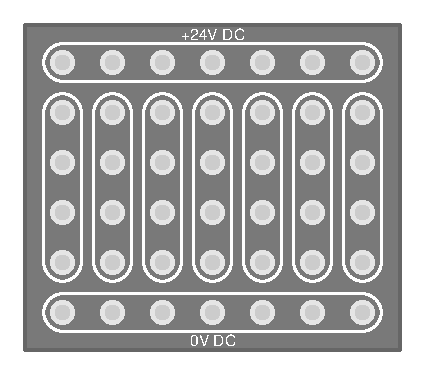
\includegraphics[width=10cm]{./koblingsbrett.eps}\includegraphics[width=4.5cm]{./multimeter.eps}$$
%\end{figure}
%\par\end{center}
%
%\subsubsection*{Utstyr du trenger}
%\begin{itemize}
%\item Labbrettet
%\item Rød og svart isolert ledning
%\item Resistans på $3.3k\Omega$ 
%\item Multimeter
%\end{itemize}
%
%\subsubsection*{Oppgaven}
%
%Du skal koble en motstand $R_{1}=3.3k\Omega$ til en likespenningskilde
%på 24VDC. På den oppkoblede kretsen skal du måle spenning over og strøm igjennom motstanden. 
%
%\begin{enumerate}
%\item Mål resistansen $R_{1}$
%\item Mål spenningen over motstanden $R_{1}$
%\item Koble inn et amperemeter og mål strømmen igjennom $R_{1}$ 
%\end{enumerate}
%
%\subsubsection*{Innlevering}
%
%Skriv en rapport for forsøket og lever på OneNote
%
%
%\newpage
%\subsubsection{LED lys og bryter}
%I denne øvingen skal du bruke koblingsbrettet til å koble en motstand
%til en spenningskilden på brettet. spenningskilden er en 230 AC til 24DC strømforsyning.   
%
%\subsubsection*{Utstyr du trenger}
%\begin{itemize}
%\item Labbrettet
%\item Rød og svart isolert ledning
%\item Resistans på $3.3k\Omega$ 
%\item Multimeter
%\end{itemize}
%
%\subsubsection*{Oppgaven}
%
%Du skal koble en bryter og et lys (LED) i serie til en likespenningskilde
%på 24VDC. På den oppkoblede kretsen skal du måle spenning over og strøm igjennom motstanden. 
%
%\begin{enumerate}
%\item Mål spenningen over motstanden $R_{1}$
%\item Mål spenningen over bryteren 
%\item Koble inn et amperemeter og mål strømmen igjennom $R_{1}$ 
%\end{enumerate}
%
%\subsubsection*{Innlevering}
%
%Skriv en rapport for forsøket og lever på OneNote
\end{document}
